\documentclass[10pt, aspectratio=169, handout]{beamer}
\usefonttheme{professionalfonts}
%\usetheme{CambridgeUS}
%
% Choose how your presentation looks.
%
% For more themes, color themes and font themes, see:
% http://deic.uab.es/~iblanes/beamer_gallery/index_by_theme.html
%
\mode<presentation>
{
  \usetheme{default}      % or try Darmstadt, Madrid, Warsaw, ...
  \usecolortheme{beaver} % or try albatross, beaver, crane, ...
  \usefonttheme{default}  % or try serif, structurebold, ...
  \setbeamertemplate{navigation symbols}{}
  \setbeamertemplate{caption}[numbered]
} 

\usepackage[english]{babel}
\usepackage[utf8x]{inputenc}
\usepackage{tikz}
\usepackage{pgfplots}
\usepackage{array}  % for table column M
\usepackage{makecell} % to break line within a cell
\usepackage{verbatim}
\usepackage{graphicx}
\usepackage{epstopdf}
\usepackage{amsfonts}
\usepackage{xcolor}
%\captionsetup{compatibility=false}
%\usepackage{dsfont}
\usepackage[absolute,overlay]{textpos}
\usetikzlibrary{calc}
\usetikzlibrary{pgfplots.fillbetween, backgrounds}
\usetikzlibrary{positioning}
\usetikzlibrary{arrows}
\usetikzlibrary{pgfplots.groupplots}
\usetikzlibrary{arrows.meta}
\usetikzlibrary{plotmarks}

\usepgfplotslibrary{groupplots}
\pgfplotsset{compat=newest} 
%\pgfplotsset{plot coordinates/math parser=false}

\usepackage{hyperref}
\hypersetup{
    colorlinks=true,
    linkcolor=blue,
    filecolor=magenta,      
    urlcolor=cyan,
}

%% 
%\def\EXTERNALIZE{1} % for externalizing figures
\input{header.tex}

\title[EE 264]{Quantization}
\author{Jose Krause Perin}
\institute{Stanford University}
\date{July 25, 2017}

\begin{document}

\begin{frame}
  \titlepage
\end{frame}

%
\begin{frame}{Outline}
\tableofcontents
\end{frame}

%
\section{Quantization in DSP}
\begin{frame}{Practice and theory}
\begin{block}{In practice}
	\begin{center}
		\resizebox{0.9\linewidth}{!}{\input{figs/adc-dsp-dac.tex}}
	\end{center}
\end{block}

\begin{block}{DSP theory}
	\begin{center}
		\resizebox{0.9\linewidth}{!}{\input{figs/ctd-lti-dtc.tex}}
	\end{center}

	\textbf{Problem:} This simplified model doesn't account for \textbf{quantization} (this lecture) or \textbf{finite precision arithmetic} (lecture 8).
\end{block}
\end{frame}

%
\begin{frame}{Including quantization}
	\begin{block}{Analog-to-digital converter}
		A more realistic model
		\begin{center}
		\resizebox{0.9\linewidth}{!}{
			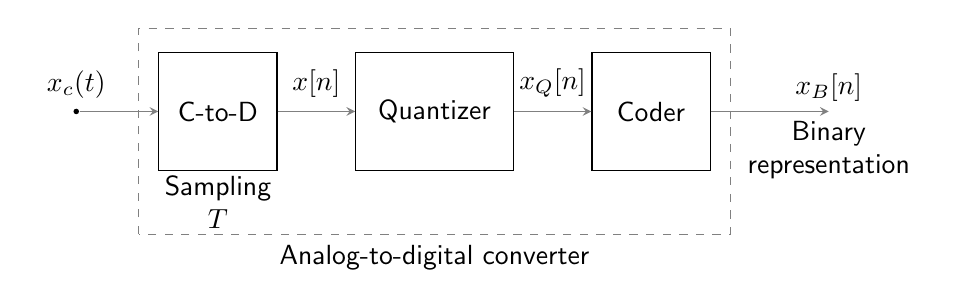
\begin{tikzpicture}[->, >=stealth, shorten >= 0pt, draw=black!50, node distance=2.75cm, font=\sffamily]
				\tikzstyle{node}=[circle,fill=black,minimum size=2pt,inner sep=0pt]
				\tikzstyle{block}=[draw=black,rectangle,fill=none,minimum size=1.5cm, inner sep=0pt]
				
				\node[node] (xc) {};
				\node[block, right=1cm of xc] (CTD) {C-to-D};
				\node[block, right of=CTD, text width = 2cm, align= center] (Q) {Quantizer};
				\node[block, right of=Q] (coder) {Coder};
				\coordinate[right=1.5cm of coder] (yc) {};
				
				\coordinate (mid1) at ($(CTD.east)!0.5!(Q.west)$) {};
				\coordinate (mid2) at ($(Q.east)!0.5!(coder.west)$) {};
				
				\path (xc) edge (CTD);
				\path (CTD) edge (Q);
				\path (Q) edge (coder);
				\path (coder) edge (yc);
				
				\node[above = 0.5mm of mid1] {$x[n]$};
				\node[above = 0.5mm of mid2] {$x_Q[n]$};
				\node[above = 0mm of xc, text width = 1cm, align=center] {$x_c(t)$};
				\node[above = 0mm of yc, align=center] {$x_B[n]$}; 
				\node[below = 0mm of yc, text width = 2.5cm, align=center] {Binary \\ representation}; 
				
				\node[align=center] at ($(CTD.south)-(0, 0.4cm)$) {Sampling \\ $T$};
				\node[align=center, text width=4cm] at ($(Q.south)-(0, 1.1cm)$) {Analog-to-digital converter};
				
				\draw[dashed] ($(CTD.south west)-(0.25, 0.8)$) rectangle ($(coder.north east)+(0.25, 0.3)$) {};
				
			\end{tikzpicture}
		}
		\end{center}
	\end{block}
\end{frame}

%
\begin{frame}{Quantizer}
	\begin{columns}[t]
		\begin{column}{0.5\textwidth}
			\textbf{Mid-tread} uniform quantizer
			\resizebox{0.9\textwidth}{!}{\input{figs/midtread_quantizer.tex}}
		\end{column}
	
		\begin{column}{0.5\textwidth}
			\textbf{Mid-rise} uniform quantizer
			\resizebox{0.9\textwidth}{!}{\input{figs/midrise_quantizer.tex}}
		\end{column}
	\end{columns}
	\begin{center}
		
	\end{center}
	
	\textbf{Terminology}
	\begin{itemize}
		\item The quantizer has $B$ bits of \textbf{resolution}
		\item $\Delta X$ is the \textbf{dynamic range}
		\item $\Delta$ is the \textbf{step size}
	\end{itemize}

	\begin{equation}
	\Delta = \frac{\Delta X}{2^{B}} \label{eq:Delta}
	\end{equation}
\end{frame}

%
\begin{frame}{Example of quantization}
\begin{center}
	\resizebox{0.5\textwidth}{!}{\input{figs/quantization_sine.tex}}
\end{center}

\onslide<2-|handout:1>{
Quantization error:
\begin{align*}
e[n] = x[n] - Q(x[n]) = x[n] - x_Q[n]
\end{align*}
Note that the quantization error is bounded $-\Delta/2 \leq e[n] \leq \Delta/2$.
}

\onslide<3-|handout:1>{
Quantization error is deterministic but hard to analyze, so we treat it as noise (random process).
}

\end{frame}

%
\begin{frame}{Quantization of a sinusoid}
	\only<1-3|handout:1>{Using a 3-bit quantizer}
	\only<4-6|handout:2>{Using an 8-bit quantizer}
	\begin{center}
		\resizebox{0.55\textwidth}{!}{\input{figs/quantization_sine_full.tex}}
	\end{center}
\end{frame}

%
\section{Linear noise model}
\begin{frame}{Linear noise model}
We'll model the quantizer as a noise source of a \textbf{white uniformly distributed noise} that is independent of the input signal. 

\begin{center}
	\resizebox{0.6\textwidth}{!}{\input{figs/quantization_linear_model.tex}}
\end{center}
\vspace{-0.5cm}
\pause
From these assumptions:
\begin{align*}
\sigma_e^2 &= \frac{\Delta^2}{12} \tag{average power} \\
\phi_{ee}[n] &= \sigma_e^2\delta[n] \tag{autocorrelation function} \\
\Phi_{ee}(e^{j\omega}) &= \sigma_e^2, |\omega| \leq \pi \tag{PSD}
\end{align*}
\end{frame}

%
\begin{frame}{Quantizer signal-to-noise ratio (SNR)}
It's often convinient to characterize the quantizer in terms of a \textbf{signal-to-noise ratio (SNR)}:
\begin{align*}
\mathrm{SNR} &= 10\log_{10}\bigg(\frac{\text{Signal Power}}{\text{Quantization noise power}}\bigg)~\text{dB} \\
&= 10\log_{10}\bigg(\frac{\sigma_x^2}{\sigma_e^2}\bigg) \\
&= 10\log_{10}\bigg(\frac{12\sigma_x^2}{\Delta^2}\bigg) \\
&= 10\log_{10}\bigg(\frac{12\sigma_x^2(2^{2B})}{\Delta X^2}\bigg) \tag{substituting \eqref{eq:Delta}} \\
&= \tikz[baseline]{\node[fill=blue!20,anchor=base] {$6.02B$};} + 10.79  + 20\log_{10}\bigg(\frac{\sigma_x}{\Delta X}\bigg) 
\end{align*}

For every bit in the quantizer we gain 6.02 dB of SNR.

\textbf{Important:} The signal amplitude must be matched to the quantizer dynamic range, otherwise there'll be excessive clipping or some of the bits may not be used. 
\end{frame}

\begin{frame}{Effective number of bits (ENOB)}

Another useful metric to evaluate quantizers is the \textbf{effective number of bits (ENOB)}.

\begin{itemize}
	\item Quantization is not the only source of noise in real quantizers
	\item Additional noise will consume some bits of resolution
	\item To continue using the simple linear noise model, we assume that the noisy real quantizer is equal to an ideal quantizer with resolution ENOB $< B$ bits.
\end{itemize}

\begin{center}
	\resizebox{0.4\textwidth}{!}{
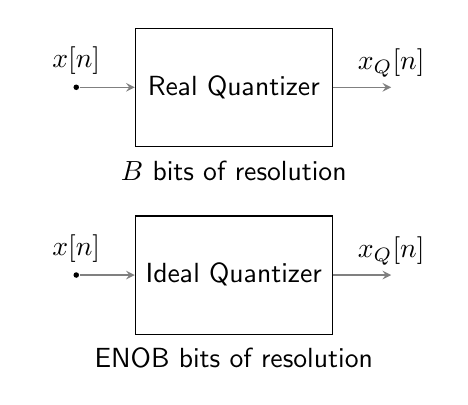
\begin{tikzpicture}[->, >=stealth, shorten >= 0pt, draw=black!50, node distance=2cm, font=\sffamily]
\tikzstyle{node}=[circle,fill=black,minimum size=2pt,inner sep=0pt]
\tikzstyle{block}=[draw=black,rectangle,fill=none,minimum size=1.5cm, inner sep=0pt]
\tikzstyle{annot} = []

\node[node] (xc) {};
\node[block, right of=xc, text width = 2.5cm, align= center] (DSP) {Real Quantizer};
\coordinate[right of=DSP] (yc) {};

\path (xc) edge (DSP);
\path (DSP) edge (yc);

\node[above = 0mm of xc, text width = 1cm, align=center] {$x[n]$};
\node[above = 0mm of yc, text width = 1cm, align=center] {$x_Q[n]$}; 
\node[align=center, text width=3cm] at ($(DSP.south) - (0, 0.3cm)$) {$B$ bits of resolution};


\node[node, below=2.3cm of xc] (xc2) {};
\node[block, right of=xc2, text width = 2.5cm, align= center] (DSP2) {Ideal Quantizer};
\coordinate[right of=DSP2] (yc2) {};

\path (xc2) edge (DSP2);
\path (DSP2) edge (yc2);

\node[above = 0mm of xc2, text width = 1cm, align=center] {$x[n]$};
\node[above = 0mm of yc2, text width = 1cm, align=center] {$x_Q[n]$}; 
\node[align=center, text width=4cm] at ($(DSP2.south) - (0, 0.3cm)$) {ENOB bits of resolution};
\end{tikzpicture}
}
\end{center}

Datasheets of ADCs will typically give you the ENOB at a certain frequency.

\end{frame}


\section{Noise shaping}
\begin{frame}{Noise shaping}

\begin{itemize}
	\item Quantization noise is unavoidable, but there are strategies to mitigate it
	\item One example is \textbf{noise shaping}. The goal is to shape the quantization noise PSD, so that most of the noise power falls outside the signal band
	\item To perform noise shaping the signal must be \textbf{oversampled}, otherwise noise aliasing would make most of the noise power fall in the signal band.
	\item Noise shaping can be used in both A-to-D and D-to-A converters
\end{itemize}
\end{frame}

\begin{frame}{Noise shaping in A-to-D conversion}
\begin{center}
	\def\ALL{1}
	\resizebox{0.6\textwidth}{!}{\input{figs/noise_shaping_adc_diagram.tex}}
\end{center}
\end{frame}

%
\begin{frame}{Noise shaping in A-to-D conversion}
\vspace{-0.3cm}
\begin{center}
	\let\ALL\undefined
	\resizebox{0.4\textwidth}{!}{\input{figs/noise_shaping_adc_diagram.tex}}
\end{center}

Using superposition, we can separately study the effect of the system on the signal $x[n]$ and on quantization noise $e[n]$. 

For the signal
\begin{align*}
Y(z) &= (X(z) - Y(z)z^{-1})\frac{1}{1 - z^{-1}} \\
Y(z)(1 - z^{-1}) &= (X(z) - Y(z)z^{-1}) \\
Y(z) &= X(z) \tag{signal is unaffected}
\end{align*}

For the noise
\begin{align*}
Y(z) &= E(z) - Y(z)\frac{z^{-1}}{1 - z^{-1}} \\
&= E(z)(1 - z^{-1}) \tag{noise is filtered}
\end{align*}
\end{frame}

%
\begin{frame}
The noise is filtered by
\begin{equation*}
\frac{Y(z)}{E(z)} = 1 - z^{-1} 
\end{equation*}
Therefore, the noise PSD at the output will be
\begin{align*}
\Phi_{\tilde{e}\tilde{e}}(e^{j\omega}) &= |1 - e^{-j\omega}|^2\sigma_e^2 \tag{since $e[n]$ is white} \\
&= 4\sigma_e^2\sin^2(\omega/2)
\end{align*}

\begin{center}
	\resizebox{0.6\textwidth}{!}{\input{figs/noise_shaping_adc_freq_domain.tex}}
\end{center}

After noise shaping most of the noise power falls out of the signal band, so we can use a simple lowpass filter to minimize quantization noise.

\pause
\textbf{Important:} This strategy of noise shaping only works when oversampling is sufficiently high. Otherwise, quantization noise would still fall in the signal band due to aliasing.
\end{frame}

%
\begin{frame}{Noise shaping in A-to-D conversion}
Table 4.1 of the textbook:

\begin{figure}[h!]
	\centering
	\includegraphics[width=0.6\textwidth]{figs/table41.png}
\end{figure}

$M$ denotes the amount of oversampling. That is $M = \frac{\text{Sampling frequency}}{\text{Nyquist frequency}}$.
\end{frame}


%
\begin{frame}{Summary}
\begin{itemize}
	\item Quantization is unavoidable in DSP systems
	\item Although quantization is a nonlinear operation on a signal, we can model the quantization error as a uniformly distributed random process (linear noise model)
	\item Using this linear noise model, we simply replace quantizers by noise sources of average power $\sigma_e^2 = \Delta^2/12$
	\item Quantization noise is assumed white (samples are uncorrelated)
	\item Every extra bit of resolution in a quantizer improves the SNR by 6.02 dB
	\item The signal amplitude must be matched to the dynamic range of the quantizer, otherwise there'll be excessive clipping or some bits won't be used
	\item Noise shaping is a strategy that minimizes quantization noise in A-to-D and D-to-A converters. The goal is to shape the quantization noise PSD, so that most of the noise power falls outside the signal band
	\item Noise shaping requires oversampling to minimize noise aliasing
\end{itemize}
\end{frame}

\end{document}
